%%%%%%%%%%%%%%%%%%%%%%%%%%%%%%%%%%%%%%%%%%%%%%%%%%%%%%%%%%%%%%%%%%%%%%%%%%%%%%%%
% Limit_Setting.tex: Limit Setting
%%%%%%%%%%%%%%%%%%%%%%%%%%%%%%%%%%%%%%%%%%%%%%%%%%%%%%%%%%%%%%%%%%%%%%%%%%%%%%%%
\chapter{Statistical Analysis}
\label{Limit_Setting}
%%%%%%%%%%%%%%%%%%%%%%%%%%%%%%%%%%%%%%%%%%%%%%%%%%%%%%%%%%%%%%%%%


%%%%%%%%%%%%%%%%%%%%%%%%%%%%%%%%%%%%%%%%%%%%%%%%%%%%%%%%%%%%%%%%%%%%%%%%%%%%%%%%
\section{Limit Computation}
%%%%%%%%%%%%%%%%%%%%%%%%%%%%%%%%%%%%%%%%%%%%%%%%%%%%%%%%%%%%%%%%%%%%%%%%%%%%%%%%
The upper limit calculation procedure used in this analysis is the CLs technique. We fed carefully estimated amounts 
of background and signal with systematic to obtain the limit.
The variable for which the 95\% upper limit is set unlike previous experiments is based entirely on the neutralino proper decay length, $c\tau_{\tilde{\chi}^{0}_{1}}$. 
%%%%%%%%%%%%%%%%%%%%%%%%%%%%%%%%%%%%%%%%%%%%%%%%%%%%%%%%%%%%%%%%%%%%%

The method we used in our upper limit calculation is by first performing a Hypothesis test and then use the result of this test to derived our confidence intervals. We do the following:
\begin{itemize}
\item We define a NULL hypothesis~($H_{0}$) and the Alternate hypothesis~($H_{1}$). If we had several other hypothesis, we will defined them also.
\item Select a Test statistics~($t(x)$), where $x$ is the data.
\item Select a corresponding test statistics calculator.
\item Use the result of the hypothesis test to compute the interval by inverting the result of the hypothesis test.
\end{itemize}
First, we describe the acceptable technique in experimental high energy physics for computing \textit{p-values} used in any search and discovery experiment.
\subsection{CLs Technique}
%%%%%%%%%%%%%%%%%%%%%%%%%%%%%%%%%%%%%%%%%%%%%%%%%%%%%%%%%%%%%%%%%%%%%
The $CL_{s}$ technique \cite{CLS} is attributed as the standard technique or framework for computing the confidence or exclusion intervals in a search and discovery experiment. It has been shown to to work during the search for the Higgs boson at LEP and recently in the discovery of the scalar boson in 2012, by both CMS and ATLAS experiments with the mass of this boson being: $m_{H} = 125.36\pm 0.37(stat.Unc)\pm0.18(syst.Unc)$.

This method has been implemented in a unique statistical software package called \textit{HiggsCombine} with the goal of providing direct access to a variety of robust statistical methods with optimised performance for computing limits or confidence intervals.
HiggsCombine \cite{LIMITS} is the official standard tool recommended by the CMS statistical committee and CMS Higgs group for calculating limits in any CMS search and discovery analysis.
It takes as input estimates on the number or distribution of signal and background and the observed number or distribution from data and produces an upper limit in the production cross section of a given physics process for a given value of a parameter of interest~(POI).
Higgscombine tool has the advantage in that, it allows for the possibility to use several different statistical methods of calculating the upper limit. This way, one can make comparison and simple checks for any inconsistency. In this analysis, we used an Asymptotic \cite{ASYMP} and HybridNew~(a hybrid of Frequentist and Bayesian methods),\cite{LIMITS}, to calculate our observed upper limits. 
%%%%%%%%%%%%%%%%%%%%%%%%%%%%%%%%%%%%%%%%%%%%%%%%%%%%%%%%%%%%%%%%%%%%
The purpose of the using the $CL_{s}$ method is to compute reliable upper limits in a search scenario when
the observed signal is very small compared to the background.
In the $CL_{s}$ technique, one uses not the p-value~($CL_{s+b}$) but rather divide this by $CL_{b}$~( which is 1 minus the $p$-value for background only hypothesis). The reason for this is to define a conditional probability conditioned to the scenario of observing only background or background only hypothesis. The $CL_{s}$ is formally defined  as:

\begin{equation}
CL_{s}  =  \frac{CL_{s+b}}{CL_{b}}  = \frac{p_{s+b}}{1 - p_{b}}
\end{equation}
where $s+b$ means signal and background.

\subsection{Statistical Test Formalism}
The Neyman-Pearson Theorem states that the likelihood ratio gives the most powerful hypothesis test. Therefore, we construct our test statistics $t_\mu$ as a function of the observed data, as a likelihood ratio.
In a search analysis, one defines the null hypothesis $H_{0}$ describing only known processes, or the background only which is to be tested against an alternate hypothesis $H_{1}$ defined as a background  and signal. However in the computation of upper limits:
\begin{itemize}
\item $H_{0}$ being the NULL hypothesis includes the background and signal~$(s + b)$ while
\item $H_{1}$ being the ALTERNATE hypothesis includes only the  background~($b$). 
\end{itemize}

Using these, two hypothesis we quantify the level of agreement between our observed data with either of the hypothesis by computing a $p$-value~($p$-value if the probability under the assumption of a given hypothesis, of finding data of equal or greater incompatibility with the predictions of the given hypothesis).
A given hypothesis is then regarded as being excluded if its $p$-value is observed below a given threshold. In particle physics, this threshold value for the $p$-value is 0.05 corresponding to 95\% of confidence level~(CL).
The CMS accepted method of computing upper upper limit is based on mix of frequentist-hybrid significance test using the profilelikelihood ratio as a test statistics~(HybridNew method). 
The parameter of interests in in our case the rate ~(cross section) of signal process as well as \textit{nuissance parameters} as systematics for the background and signal models. This parametrized systematics effects results, as is always the case, to loss in sensitivity.

In this search experiment, for each event in the signal, we measured the timing of the photon as our observable. We use this value to construct a histogram $\mathbf{n} = \left( n_{1}, \cdots, n_{N}\right)$. The expectation value for each value of $n_{i}$ can be written as:
\begin{equation}
 E[n_{i}] = \mu s_{i} + b_{i}
\end{equation}
where $\mu$ is the parameter which determines the signal strength, when $\mu = 0$ means background-only and when $\mu=1$ then we have the signal and background hypothesis. The the mean number of entries in the $i$th bin from signal and background are given as:
\begin{equation}
s_{i} = s_{tot} \int_{bin, i} f_{s}\left(t;\mathbf{\theta_{s}}\right) \quad 
b_{i} = b_{tot} \int_{bin, i} f_{b}\left(t;\mathbf{\theta_{b}}\right)
\end{equation}
with the functions $f_{s}\left(t;\mathbf{\theta_{s}}\right) $ and $f_{b}\left(t;\mathbf{\theta_{b}}\right) $ being the probability density functions~(Pdfs) of the variable $t$ for the signal and background events and $\mathbf{\theta_{s}} $ and $\mathbf{\theta_{b}} $ representing the parameters which characterise the shapes of the pdfs. $s_{tot}$ and $b_{tot}$ represents the total mean numbers of signals and backgrounds while the integrals represent the probabilities for an event to be found in bin $i$. $\mathbf{\theta} = \left( \mathbf{\theta_{s}}, \mathbf{\theta_{b}}, b_{tot} \right)$ denote all nuisance parameters~(systematic uncertainties) while $s_{tot}$ is the signal normalization is fixed to the value predicted by the nominal signal model.

The likelihood function is the product of the Poisson probabilities for all bins:
\begin{equation}\label{eq:LL}
\mathcal{L}\left( \mu, \mathbf{\theta} \right) = \prod^{N}_{r=1} \frac{{\left( \mu s_{r} + b_{r} \right)}^{n_{r}}}{n_{r}!} e^{-(\mu s_{r} + b_{r})} \cdot \mathcal{G}(\mathbf{\theta} )
\end{equation}
where $\mathcal{G}(\mathbf{\theta} )$ is a discrete~(Poisson) distribution of the nuisance parameters. This distribution can be different for different nuisance parameter.

Using the likelihood function, the profilelikelihood ratio is then defined as:
\begin{equation}\label{eq:PLL}
\lambda(\mu) =  \frac{\mathcal{L}(\mu, \hat{\hat{\mathbf{•\theta}}})}{\mathcal{L}(\hat{\mu}, \hat{\mathbf{\theta}} )}
\end{equation}
Here $\hat{\hat{\mathbf{•\theta}}} $ is the the value of $\mathbf{\theta}$ that maximizes $\mathcal{L}$ for a specified $\mu$, thus, it is referred to as the \textit{conditional maximum-likelihood estimator}~(CMLE) of $\mathbf{\theta}$ (given as a function of $\mu$). While $\mathcal{L}(\hat{\mu}, \hat{\mathbf{\theta}} )$ is the maximized (unconditional) likelihood function with $\hat{\mu}$ and $\hat{\mathbf{\theta}}$ being its \textit{maximum likelihood}~(ML) estimators.
The nuisance parameters broadens the profilelikelihood as a function of $\mu$ relative to what is expected if their values where fixed and this reflects in the loss of sensitivity or information about $\mu$ due to the systematic uncertainties.
\subsection{Test Statistics and $p$-values}
\par
The above expression for $\lambda(\mu)$ shows that $0 \leq \lambda \leq 1$, where $\lambda$ close to 1 indicates a very good agreement between the data and hypothesis value of $\mu$.
The test statistics  to be used for our statistical test is defined as:
\begin{equation}
 t_{\mu} = -2\ln \lambda(\mu)
\end{equation}
It is important to note that the test statistics approach to any statistical test is favourable because just be looking at the values of the test statistics, higher values corresponds to increasing incompatibility between the data and the value of $\mu$ which is from the signal hypothesis. 
This incompatibility or disagreement between the data and a given hypothesis is quantified by calculating the probability or $p$-value as:
\begin{equation}
 CL_{s+b} = p_{u} = \int^{\infty}_{t_{\mu,obs}} f(t_{\mu}|\mu) dt_{\mu}
\end{equation}
where, $t_{\mu,obs}$ is the value of the test statistics $t_{\mu}$ obtained from the data and $f(t_{\mu}|\mu)$ is a pdf constructed from $t_{\mu}$ depending on the signal strength $\mu$.
The set of values for $\mu$ that a rejected because their $p$-value is below a specified threshold value $\alpha$
lying on either sides of those not rejected gives a two sided confidence interval of $\mu$ and if just on one side of the ones not rejected gives an upper limit on the rejected values of $\mu$.

In the background only scenario i.e $\mu = 0$, the test statistics is defined as:

%\begin{equation}\label{eq:HNULL}
\[\label{eq:HNULL}
 q_{\mu} = \left\lbrace  
  \begin{array}{ll}
 -2\ln \lambda(0), & \hat{\mu} \geq 0 \\
   0,              & \hat{\mu} \leq 0
  \end{array}
  \right.
\]

where $\lambda(0)$ is the profilelikelihood ratio for $\mu = 0$  defined in \ref{eq:PLL}.
and again to quantify the disagreement between the background-only hypothesis~($\mu = 0$) and the data is given by the $p$-value as:
\begin{equation}
 CL_{b} = p_{0} = \int^{\infty}_{q_{0,obs}} f(q_{0}|0) dq_{0}
\end{equation}
where $f(q_{0}|0)$ denotes the pdf if the test statistics $q_{0}$ under the background-only~($\mu = 0$) hypothesis.
Figure \ref{fig:LIM} shows a sampling distributions of the test statistics and how the $p$-values can be extracted from these distributions.

\begin{center}
\centering
%\mbox{
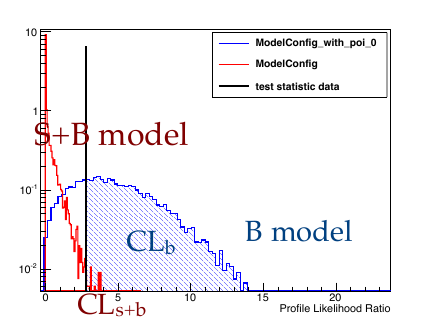
\includegraphics[height=2.2in]{THESISPLOTS/Asymptotics_Test_Stats.png}
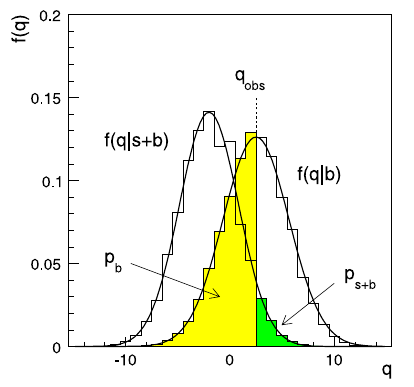
\includegraphics[scale=0.6]{THESISPLOTS/TEST_STATISTICS.png}
\captionof{figure}{Sampling distributions for $f(t_{\mu}|\mu)$ showing how one extracts the $p$-vlaues. left: is the using a analytic of the Asymptotic method and right: is from the HybridNew method.}
\label{fig:LIM}
\end{center}


\par In addition to the $p$-value, for expressing the disagreement between the data and a given hypothesis, the Higgscombine tool also provides a quantity known as the \textit{significance}~($\mathcal{Z}$). $\mathcal{Z}$ and the $p$-value have a very non-linear relation. Once can defined that relation using a two-sided fluctuation if a Gaussian variable $\sigma$, with $5\sigma$ significance corresponding to a $p$-value of $p = 5.7 \times 10^{-7}$ to denote a discovery. Since, we have not observed any significant excess of events over our standard model background, we will not mention a lot about significance in this thesis, but rather talk about $p$-values as they are indispensable in computing limits.

The important question is always, how does one obtain an expression or a distribution of the test statistics and $f(t_{\mu}|\mu)$ from the likelihood function? To answer this question, the HiggsCombine tool was developed which consist of various ways of both analytically~(e.g the Asymptotic statistical method \cite{ASYMP}) or through numerical integration or Monte Carlo computation~( e.g the HybridNew statistical method) obtain the test statistics and $ f(t_{\mu}|\mu)$. We have shown the limit computation results of both methods as used in this analysis.
As an example, the pdf $ f(q_{\mu}|\mu)$ of the test statistics~($q_{\mu}$) obtained though the \textcolor{green}{Asymptotic} statistical method as given in \cite{ASYMP} is:
\begin{equation}\label{eq:ASYPTOTIC}
f(t_{\mu}|{\mu}^{\prime}) = \mathbf{\Phi}\left( \frac{\mu -{\mu}^{\prime}}{\sigma}\right)\delta(t_{\mu}) +
                             \frac{1}{2}\frac{1}{\sqrt{2\pi}}\frac{1}{t_{\mu}}\exp\left[-\frac{1}{2} \left(  \sqrt{t_{\mu}} - \frac{\mu - {\mu}^{\prime}}{\sigma}\right)^{2} \right]
\end{equation}
where result to a half-chi-square distribution when $\mu = \mu^{\prime}$.

In subtle point worth mentioning is that in the HybridNew approach, systematics uncertainties are taken into account through the Beyesian prior density $\mathbf{\pi(\theta)}$, and the distribution of the test statistics is computed under the assumption if the Beyesian model of average given as: $$\displaystyle{f(q) = \int f(q|\theta)\pi(\theta)d\theta}$$ and the prior pdf $\mathbf{\pi(\theta)}$ is obtained from some measurements characterised by a given likelihood function $\mathcal{L}_{\mathbf{\theta}}(\mathbf{\theta} )$ which is then used to find the prior using Bayes' Theorem. Unlike other cases where systematic uncertainties are taking as being part of the data and incorporated directly through $\mathcal{G}(\theta)$ as shown in equation \ref{eq:LL}. Nevertheless, they arrive at the same result.

\par
In summary, the hypothesis test is performed using a given statistical method on each value of a chosen parameter of interest~(POI)(usually denoted $\mu$). The $p$-value if obtained from the sampling distribution of the test statistics being used. Can either obtain this test statistics analytically or through Monte Carlo computation and  numerical integration. By plotting the p-value as a function of the POI, we obtain the p-value curve~(in this case the $CL_{s} = \frac{CL_{s+b}}{CL_{b}}$).
The value of $\mu$ which has a p-value $\alpha$~( e.g $0.05$) is the upper limit~(for 1-dimensional limits,2-dimensional limits gives lower and upper limits) of $1 - \alpha$  confidence interval~(e.g 95\%).
\begin{center}
\centering
%\mbox{
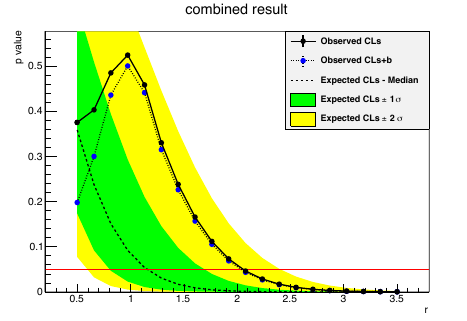
\includegraphics[scale=1.0]{THESISPLOTS/Limits_CLs.png}
\captionof{figure}{Distribution of $p$-vlaues showing how upper limit on $\mu$ is extracted for a given threshold probability.}
\label{fig:LIMITS_CLS}
\end{center}

